\documentclass[10pt,a4paper,twocolumn]{article}
\usepackage[utf8]{inputenc}
\usepackage[T1]{fontenc}
\usepackage{graphicx}
\graphicspath{{./figures/}}
\usepackage{amsmath}
\usepackage{amsfonts}
\usepackage{amssymb}
\usepackage[left=1.5cm, right=1.5cm, top=2.50cm, bottom=2.50cm]{geometry}
\usepackage{multicol}
\usepackage{float}

\author{Fabian Schubert}
\title{Nonlinear Dendritic Coincidence Detection for Supervised Learning}

\usepackage[numbers]{natbib}
\bibliographystyle{abbrvnat}

\renewcommand{\arraystretch}{1.5}

\usepackage{layouts}


\begin{document}
	\maketitle

		\section{Introduction}
		
		In recent years, a growing body of research has addressed the 
		functional implications of the distinct physiology and anatomy of 
		cortical pyramidal neurons \cite{Spruston2008,Hay2011,Ramaswamy2015}. 
		In particular, on the theoretical side,
		we saw a paradigm shift from treating neurons as point-like electrical
		structures towards embracing the entire dendritic structure 
		\cite{Larkum2009,Poirazi2009,Shai2015}. This was 
		mostly due to the fact that experimental work uncovered dynamical properties
		of these cells that simply could not be accounted for by point models
		\cite{Spruston1995,Hausser2000}.
		
		An important finding was that the apical dendritic tree of
		cortical pyramidal neurons can act as a separate nonlinear synaptic 
		integration zone \cite{Spruston2008,Branco2011}. 
		Under certain conditions, a dendritic $\rm Ca^{2+}$ spike
		can be elicited that propagates towards the soma, causing rapid, bursting
		spiking activity. One of the cases in which dendritic spiking can occur
		was termed `backpropagation-activated $\rm Ca^{2+}$ spike firing' 
		(`BAC firing'): A single somatic spike can backpropagate towards the apical
		spike initiation zone, in turn significantly facilitating the initiation of 
		a dendritic spike \cite{Stuart2001,Spruston2008,Larkum2013}. 
		This reciprocal coupling is believed to act as a form of
		coincidence detection: If apical and basal synaptic input co-occurs, the 
		neuron can respond with a rapid burst of spiking activity. The firing rate
		of these temporal bursts exceeds the firing rate that is maximally achievable 
		under basal synaptic input alone, therefore representing a form of temporal coincidence
		detection between apical and basal input.
		
		Naturally, these mechanisms also affect plasticity and thus learning
		within the cortex \cite{Sjoestroem2006,Ebner2019}. 
		While the interplay between basal and apical stimulation and
		its effect on synaptic efficacies is subject to ongoing research, there is
		some evidence that BAC-firing tends to shift plasticity towards long-term potentiation
		(LTP) \cite{Letzkus2006}. 
		Thus, coincidence between basal and apical input appears to also gate synaptic
		plasticity.
		
		In a supervised learning scheme, where the top down input
		arriving at the apical compartment acts as the teaching signal,
		the most straight-forward learning rule for the basal synaptic
		weights would be derived from an appropriate loss function,
		such as a mean square error, based on the difference between 
		basal and apical input, i.e.\ $I_{\rm p} - I_{\rm d}$. Theoretical work has 
		investigated possible learning mechanisms
		that could utilize an intracellular error signal
		\citep{Urbanczik_2014,Schiess_2016,Guerguiev_2017}.
		However, a clear experimental
		evidence for a physical quantity encoding such an error 
		is---to our knowledge---yet to be found. 
		On the other hand, Hebbian-type plasticity is extensively
		documented in experiments. Therefore, our work is
		based on the question whether the non-linear interactions
		between basal and apical synaptic input could, when
		combined with a Hebbian plasticity rule, allow a neuron
		to learn to reproduce an apical teaching signal in its
		proximal input.
		
		In our work, we combine a phenomenological model that generates the output
		firing rate as a function of two streams of synaptic input (subsuming basal and apical input)
		with Hebbian, as well as BCM-like plasticity rules on basal synapses. We hypothesized that 
		this combination of neural activation and plasticity rules would lead to an
		increased correlation between basal and apical input.
		
		Furthermore, this temporal alignment could potentially facilitate apical inputs to act
		as top-down teaching signals, without the need for an explicit error-driven
		learning rule. Thus, we also test our model in a simple linear 
		supervised classification task and compare it with the performance of a simple
		point neuron equipped with similar plasticity rules.
		
		\section{Model}
		
		\subsection{Neuron Model}
		
		The neuron model used throughout this study is a discrete-time rate encoding model that
		uses two separate input variables, subsuming the total synaptic
		input current injected arriving at the basal (proximal) and apical (distal) 
		dendritic structure of a pyramidal neuron, respectively. The model is a slightly
		simplified version of a phenomenological model proposed by \citet{Shai_2015}.
		Denoting the input currents by $I_{\rm p}$ (proximal) and $I_{\rm d}$ (distal), 
		the model is written as
		%%%%%%%%%%%%%%%%%%%%%%%%%%%%%%%%%%%%%
		\begin{align}
		\begin{split}
		y\left(t\right) &= \sigma\left( I_{\rm p}(t) - \theta_{p0} \right)
		\left[1-\sigma\left(I_{\rm d}(t) - \theta_d\right)\right] \\
		&+ \alpha \sigma\left(I_{\rm d}(t) - \theta_d \right)\sigma\left( I_{\rm p}(t) - \theta_{p1} \right)
		\end{split} \label{eq:comp_model}\\
		\sigma(x) &\equiv \frac{1}{1+\exp(-4x)} \; .
		\end{align}
		%%%%%%%%%%%%%%%%%%%%%%%%%%%%%%%%%%%%%
		Here, $\theta_{p0}$, $\theta_{p1}$ and $\theta_d$ are threshold variables with
		respect to proximal and distal input. Overall, this equation describes two distinct
		regions of neural activation in the $(I_{\rm p}, I_{\rm d})$-space which differ in their
		maximal firing rates, which are set to $1$ and $\alpha$, where $0 < \alpha < 1$.
		A plot of \eqref{eq:comp_model} is shown in Fig.~\ref{fig:comp_model}.
		%%%%%%%%%%%%%%%%%%%%%%%%%%%%%%%%%%%%%
		\begin{figure}
			\centering
			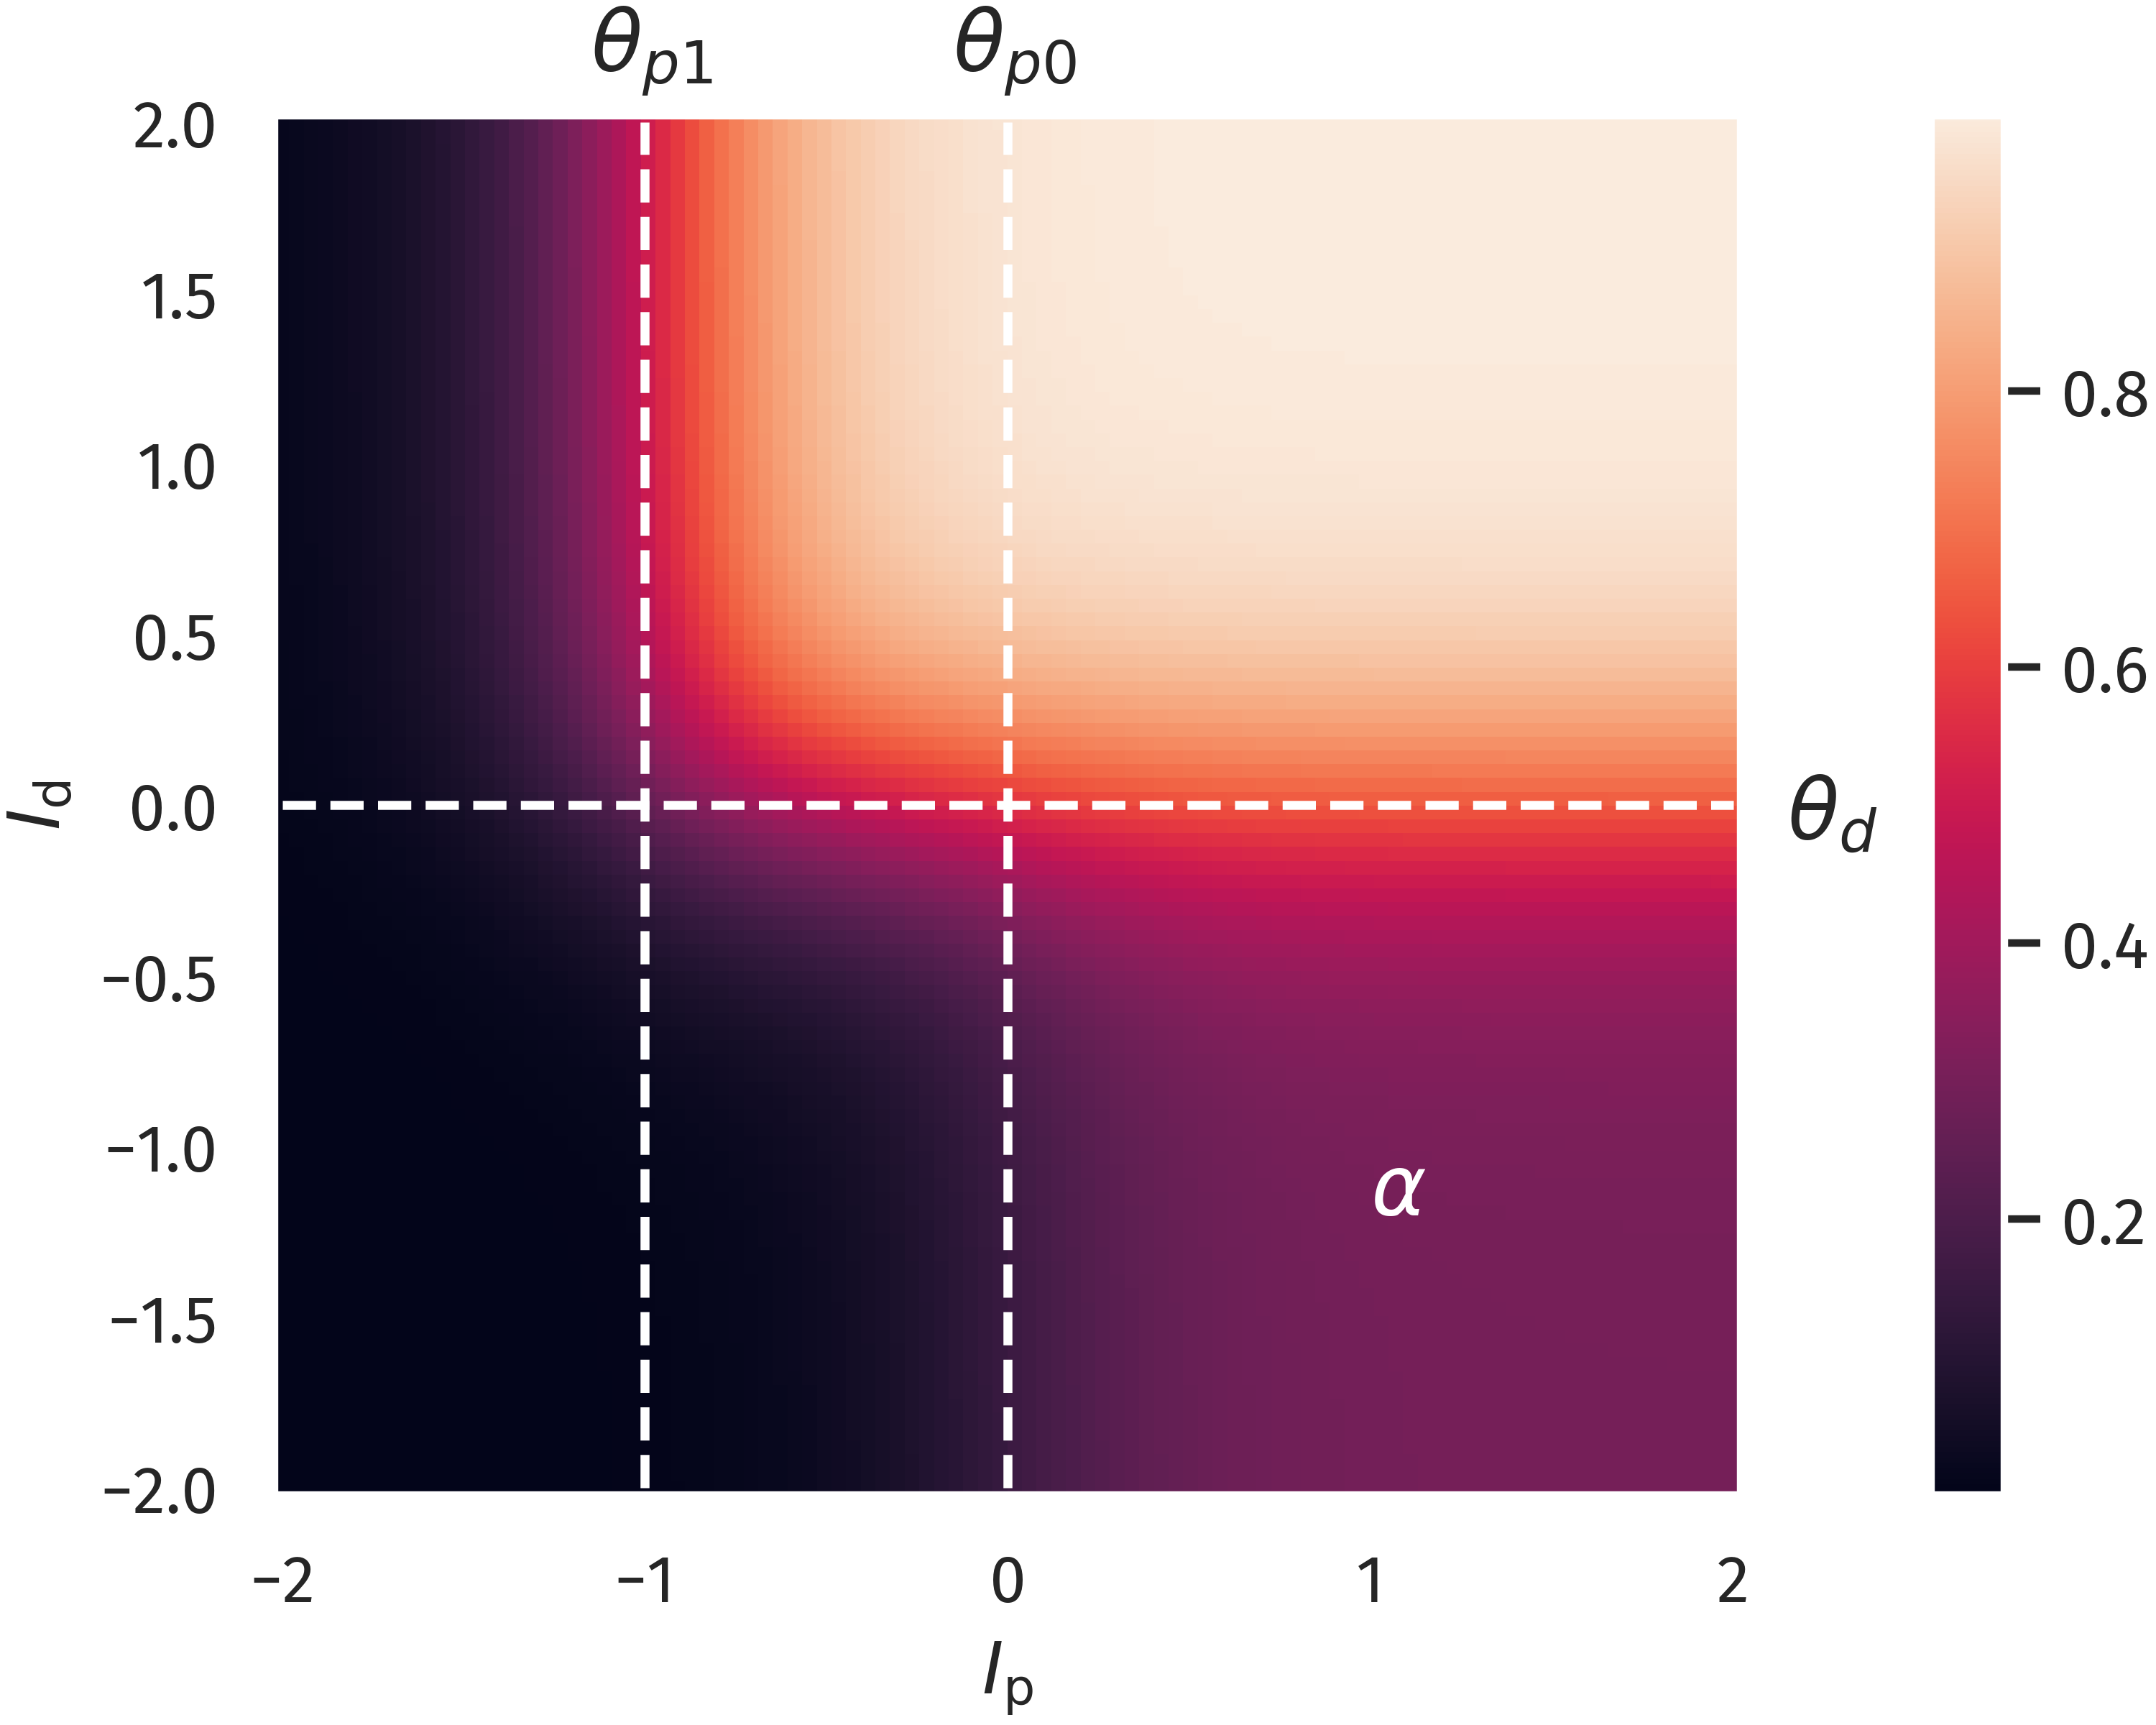
\includegraphics[width=0.8\columnwidth]{plot_comp_mod_marks.png}
			\caption{{\bf Two-compartment rate model.} Firing rate as a
			function of proximal and distal input $I_{\rm p}$ and $I_{\rm d}$, 
			see \eqref{eq:comp_model}. 
			The thresholds $\theta_{p0}$, $\theta_{p1}$ and $\theta_d$ define
			two regions of neural activity with a a maximal firing rate of $1$
			and $\alpha$.}
			\label{fig:comp_model}
		\end{figure}
		%%%%%%%%%%%%%%%%%%%%%%%%%%%%%%%%%%%%%
		
		In all our numerical experiments, we compare this model with a 
		simple point neuron model that was given by
		%%%%%%%%%%%%%%%%%%%%%%%%%%%%%%%%%%%%%
		\begin{equation}
			y(t) = \sigma\left(I_{\rm p}(t) + I_{\rm d}(t) - \theta \right) \; .
		\end{equation}
		%%%%%%%%%%%%%%%%%%%%%%%%%%%%%%%%%%%%%
		The apical input $I_{\rm d}$ was generated
		`as is', meaning, it is not dynamically calculated as a superposition
		of multiple presynaptic inputs, but given by
		%%%%%%%%%%%%%%%%%%%%%%%%%%%%%%%%%%%%%
		\begin{equation}
			I_{\rm d}(t) = n_d(t) x_d(t) - b_d(t) \; ,
			\label{eq:I_d}
		\end{equation}
		%%%%%%%%%%%%%%%%%%%%%%%%%%%%%%%%%%%%%
		where $n_d(t)$ is a scaling factor, $x_d(t)$ a pre-generated
		discrete time sequence and $b_d(t)$ a bias. Note that $n_d$ and $b_d$ 
		are time dependent since they are subject to adaptation processes 
		that are described in the next section.
		
		Similarly, $I_{\rm p}(t)$ is given by
		%%%%%%%%%%%%%%%%%%%%%%%%%%%%%%%%%%%%%
		\begin{equation}
			I_{\rm p}(t) = n_p(t) \sum_{i=1}^{N} x_{p,i}(t) w_i(t) - b_p(t) \; ,
		\end{equation}
		%%%%%%%%%%%%%%%%%%%%%%%%%%%%%%%%%%%%%
		where $N$ is the number of presynaptic afferents, $x_{p,i}(t)$ the
		corresponding sequences and $w_i(t)$ the synaptic efficacies.
		As for $I_{\rm d}(t)$, $n_p(t)$ and $b_p(t)$ is a time dependent
		scaling and bias.
		
		\subsection{Plasticity}
		
		We implemented a Hebbian plasticity rule for the basal 
		synaptic weights given by the following update equation:
		%%%%%%%%%%%%%%%%%%%%%%%%%%%%%%%%%%%%%
		\begin{align}
			w_i(t+1) &= w_i(t) + \mu_w \left(x_{p,i}(t) - \tilde{x}_{p,i}(t)\right)
			\left(y(t) - \tilde{y} \right)
			\label{eq:bcm_plast} \\
			\tilde{x}_{p,i}(t+1) &= (1-\mu_{av})\tilde{x}_{p,i}(t) + \mu_{av}x_{p,i}(t+1) \\
			\tilde{y}(t+1) &= (1-\mu_{av})\tilde{y}(t) + \mu_{av}y(t+1)
		\end{align}
		%%%%%%%%%%%%%%%%%%%%%%%%%%%%%%%%%%%%%
		Additionally, we use a
		synaptic normalization constraint
		%%%%%%%%%%%%%%%%%%%%%%%%%%%%%%%%%%%%%
		\begin{equation}
			w_i(t) \rightarrow \frac{w_i(t)}{\lVert \mathbf{w}(t)\rVert}
			\label{eq:weight_norm}
		\end{equation}
		%%%%%%%%%%%%%%%%%%%%%%%%%%%%%%%%%%%%%
		in each time step, where $\lVert \mathbf{w}(t)\rVert$ denotes the Euclidean
		norm of the synaptic weight vector. 
%		The threshold $\theta_y$ was
%		chosen such that LTP is present if neural activity is in the
%		high-activity regime (yellow area in Fig.~\ref{fig:comp_model}), while
%		LTD is present in the low-activity regime 
%		(given by $\alpha$, see Fig.~\ref{fig:comp_model}). Hence, we set
%		$\theta_y = (1+\alpha)/2$.
		
		For comparative reasons, the point neuron model is equipped with the
		same plasticity rule for the proximal weights as \eqref{eq:bcm_plast}. 
%		except that the threshold $\theta_y$ was dynamically adjusted as
%		%%%%%%%%%%%%%%%%%%%%%%%%%%%%%%%%%%%%%
%		\begin{equation}
%			\theta_y(t+1) = \left(1-\mu_{av}\right)\theta_y(t) + \mu_{av} y^2(t) \; , 
%		\end{equation}
%		%%%%%%%%%%%%%%%%%%%%%%%%%%%%%%%%%%%%%
%		which is an implementation of a running average of the square activity,
%		as used in the classic BCM-rule.
		
		Additionally, the scaling and bias variables are changing dynamically
		according to the following homeostatic plasticity rules:
		%%%%%%%%%%%%%%%%%%%%%%%%%%%%%%%%%%%%%
		\begin{align}
			b_p(t+1) &= b_p(t) + \mu_b \left[I_{\rm p}(t) - I_{\rm p}^t\right] \\
			b_d(t+1) &= b_d(t) + \mu_b \left[I_{\rm d}(t) - I_{\rm d}^t\right] \\
			n_p(t+1) &= n_p(t) + \mu_n \left[V_p^t - \left( I_{\rm p}(t) - \tilde{I}_p(t)\right)^2\right] \\
			n_d(t+1) &= n_d(t) + \mu_n \left[V_d^t - \left( I_{\rm d}(t) - \tilde{I}_d(t)\right)^2\right] \\
			\tilde{I}_p(t+1) &= (1-\mu_{av})\tilde{I}_p(t) + \mu_{av} I_{\rm p}(t+1) \\
			\tilde{I}_d(t+1) &= (1-\mu_{av})\tilde{I}_d(t) + \mu_{av} I_{\rm d}(t+1)
		\end{align}
		%%%%%%%%%%%%%%%%%%%%%%%%%%%%%%%%%%%%%
		Here, $I_{\rm p}^t$, $I_{\rm d}^t$, $V_p^t$ and $V_p^t$ define targets for the 
		temporal means and variances of $I_{\rm p}$ and $I_{\rm d}$. The dynamic variables 
		$\tilde{I}_p$ and $\tilde{I}_d$ are simply low-pass filtered running 
		averages of $I_{\rm p}$ and $I_{\rm d}$.
		
		A list of all parameter values is given in Table~\ref{tab:parameters}.
		
		%%%%%%%%%%%%%%%%%%%%%%%%%%%%%%%%%%%%%
		\begin{table}
			\begin{tabular}{ l | l || l | l }
				$\theta_{p0}$ & $0$ & $V_d^t$ & $0.25$ \\
				$\theta_{p1}$ & $-1$ & $\mu_b$ & $10^{-3}$ \\ 
				$\theta_{d}$ & $0$ & $\mu_n$ & $10^{-4}$ \\  
				$\alpha$ & $0.3$ & $\mu_{av}$ & $5 \cdot 10^{-3}$ \\   
				$\mu_w$ & $5 \cdot 10^{-5}$ & $I_{\rm p}^t$ & $0$ \\
				$V_p^t$ & $0.25$ & $I_{\rm d}^t$ & $0$  
			\end{tabular}
		\caption{Model parameters}
		\label{tab:parameters}
		\end{table}
		%%%%%%%%%%%%%%%%%%%%%%%%%%%%%%%%%%%%%
		
		\section{Results}
		\label{sect:results}
		
		\subsection{Increased Alignment between Basal and Apical Inputs}
		\label{sect:alignment}
		
		As a first test, we wanted to quantify the neuron's ability to 
		align its basal input to the apical teaching signal.
		To do so, we defined the pearson correlation coefficient
		$\rho[I_{\rm p},I_{\rm d}]$ between the basal and apical input current
		as our measure of interest. We determined this temporal
		correlation coefficient after simulating all plasticity mechanisms
		under stationary random input sequences with certain statistical
		properties that shall be explained in the following.
		As a starting point, we chose all $x_{p,i}(t)$ to be randomly
		drawn from a uniform distribution, where $x_{p,i}(t) \in (0,1)$.
		For $I_{\rm d}(t)$ to be fully `reconstructable' by the basal input, 
		$x_d(t)$ had to be some linear combination of all $x_{p,i}(t)$.
		Therefore, we chose $x_d(t) = \sum_{i=1}^N a_i x_{p,i}(t)$, where
		$\mathbf{a}$ is a random vector with unit length.
		Since we used a Hebbian learning scheme, we expected that 
		the direction and magnitude of the principal components of 
		the basal input would also significantly affect the outcome of
		the experiment: A large variance in the basal input 
		orthogonal to the `reconstruction vector' $\mathbf{a}$ 
		should act as a distraction for the plasticity and reduce the
		resulting alignment between $I_{\rm p}$ and $I_{\rm d}$. Therefore, we 
		applied a transformation to the input sequences $x_{p,i}(t)$
		that were parameterized by two quantities, a scaling factor $s$
		and the dimension $N_{dist}$ of a subspace of the basal input space.
		A set of $N_{dist}$ orthonormal basis vectors was randomly generated,
		which were also orthogonal to $\mathbf{a}$. Withing this $N_{dist}$-dimensional
		subspace, the input sequences $x_{p,i}(t)$ were then rescaled by the
		factor $s$. 
		
		After both $x_{p,i}(t)$ and $x_d(t)$ were generated,
		a simulation was run using all previously described plasticity
		mechanisms until the dynamic variables reached a stationary state.
		After this learning phase, another set of input sequences was generated
		using the previously described protocol and $\rho[I_{\rm p},I_{\rm d}]$ was calculated.
		Note that plasticity was turned off in this phase. This entire procedure
		allowed us to calculate $\rho[I_{\rm p},I_{\rm d}]$ as a function of the distraction
		parameters $s$ and $N_{dist}$. The results for both neuron models 
		is shown in Fig.~\ref{fig:corr_dimension_scaling}. Here, the total number of 
		basal inputs is $N=10$. One can observe a decorrelation transition for 
		both models. However, the compartment model supports a significantly stronger
		distraction in terms of the scaling factor $s$ as compared to the point model.
		This is a first confirmation of our hypothesis that nonlinear interactions
		between basal and apical input could improve learning guided by top-down signals.
		
		%%%%%%%%%%%%%%%%%%%%%%%%%%%%%%%%%%%%%
		\begin{figure}
			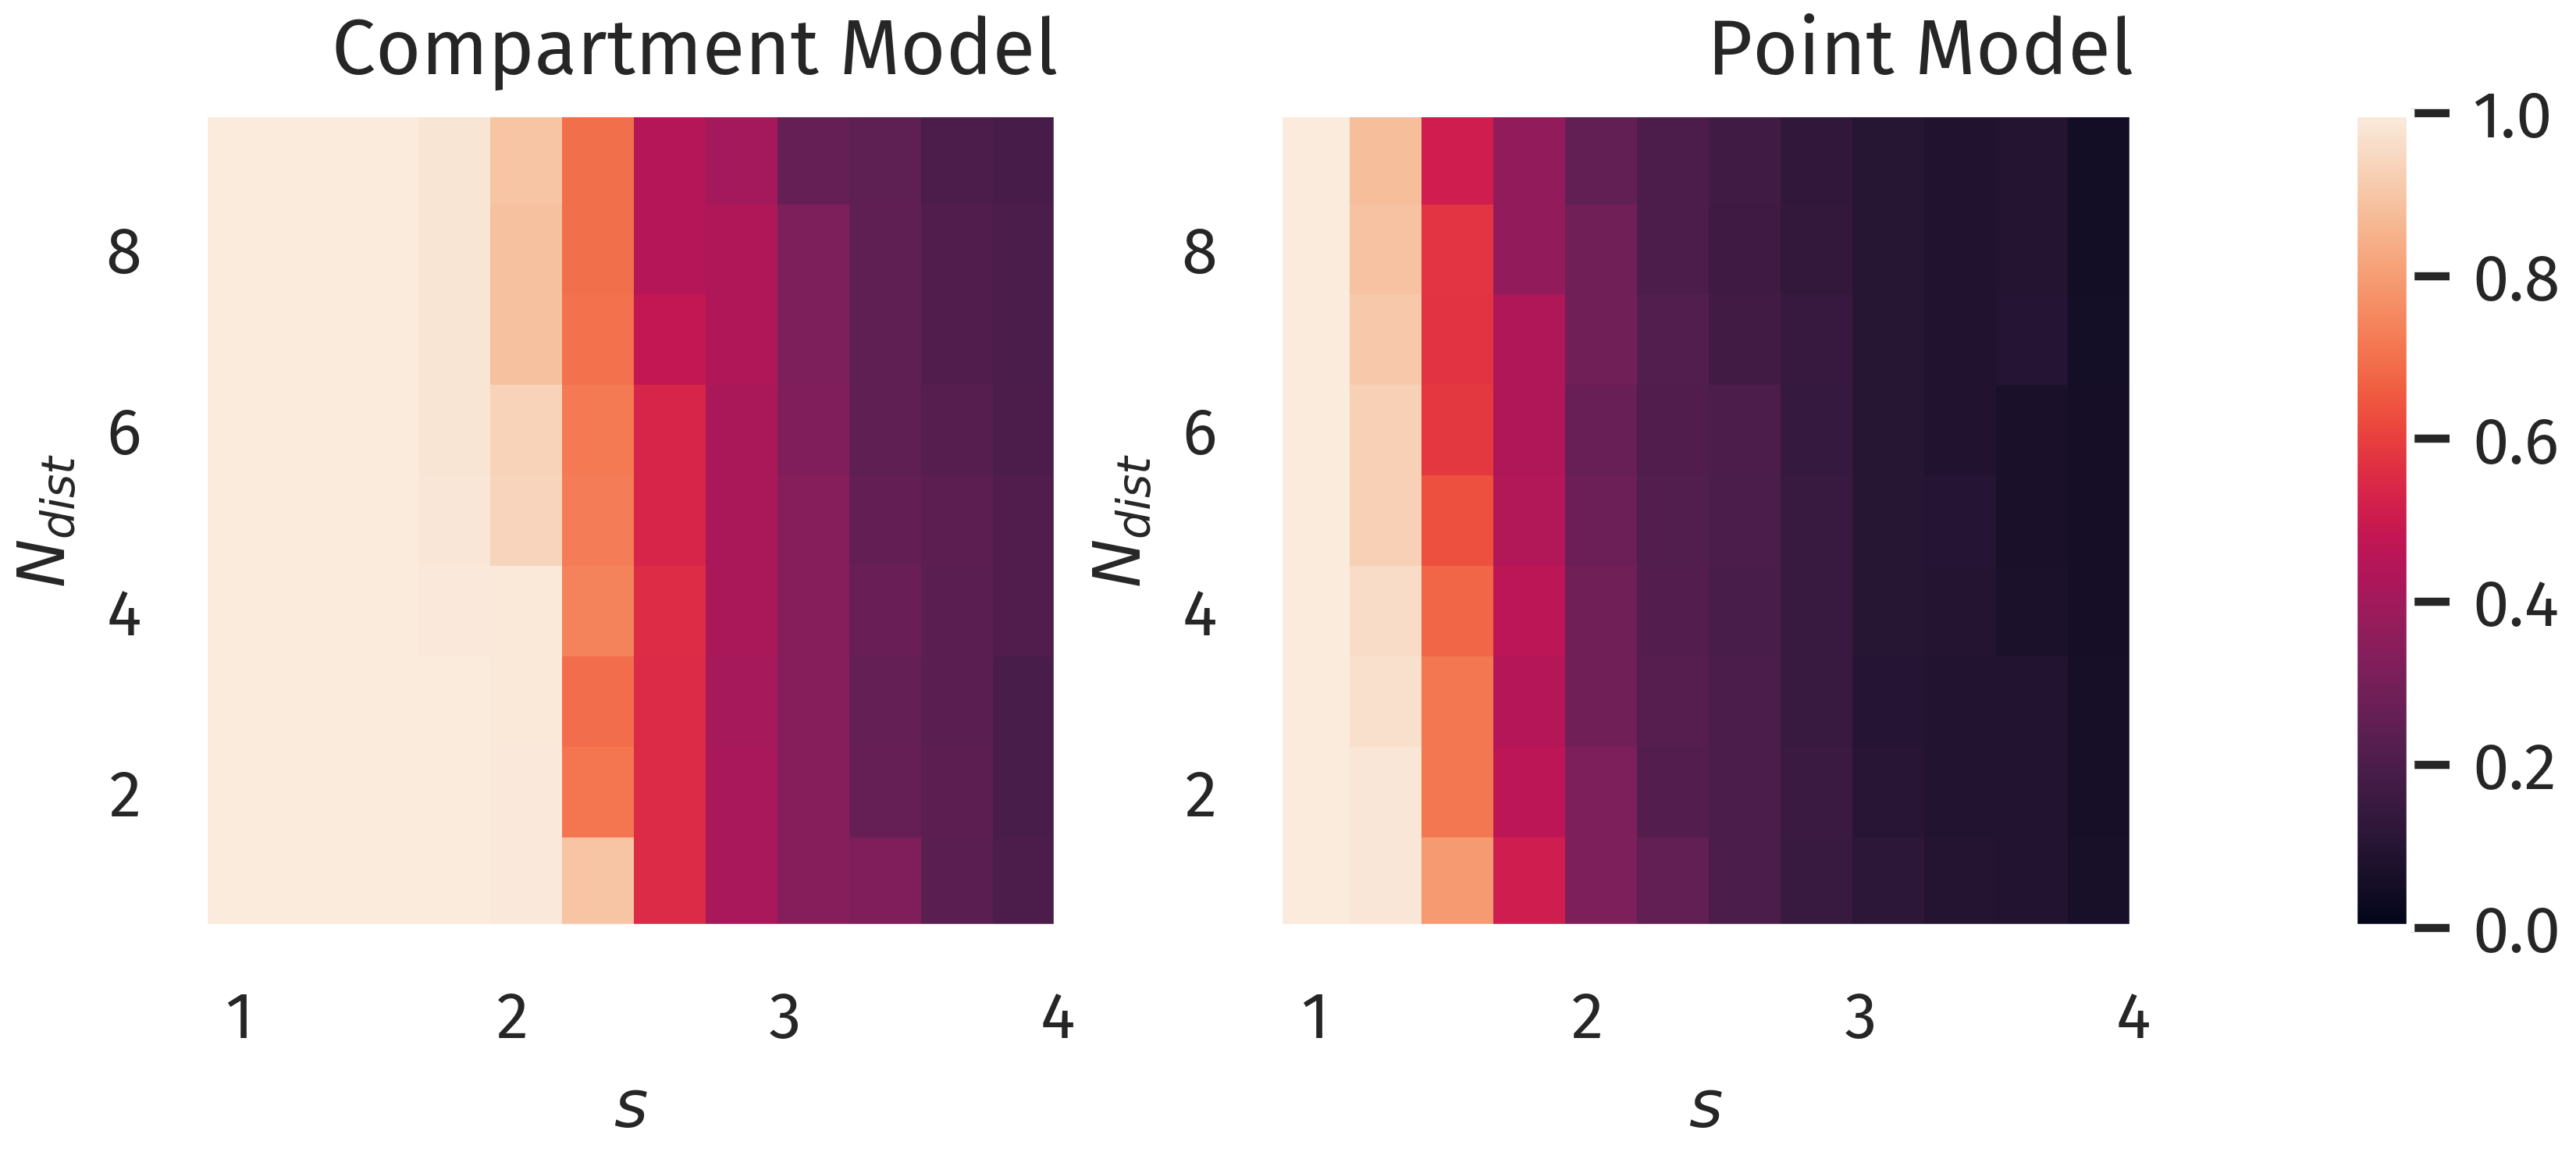
\includegraphics[width=\columnwidth]{corr_dimension_scaling}
			\caption{{\bf Alignment between Basal and Apical Input.} Color
			encodes the Pearson correlation $\rho[I_p,I_d]$ for different
			number of orthogonal distraction directions $N_{dist}$ 
			and the corresponding scaling faction $s$.}
			\label{fig:corr_dimension_scaling}
		\end{figure}
		%%%%%%%%%%%%%%%%%%%%%%%%%%%%%%%%%%%%%
		
		\subsection{Supervised Learning in a Linear Classification Task}
		\label{sect:classification}
		
		Next, we investigated if the observed differences would also improve
		the performance in an actual supervised learning task.
		For this purpose, we constructed presynaptic basal input as illustrated
		in Fig.~\ref{fig:illustration_classification}.
		Written in vector form,
		each sample from the basal input is generated from the following expression:
		%%%%%%%%%%%%%%%%%%%%%%%%%%%%%%%%%%%%%
		\begin{equation}
			\mathbf{x}_p(t) = \mathbf{b} + \mathbf{a}\left(c(t) + \sigma_a \zeta_a(t) \right) 
			+ s \cdot \sum_{i=1}^{N_{dist}} \zeta_{dist,i}(t) \mathbf{v}_{dist,i} \; .
		\end{equation}
		%%%%%%%%%%%%%%%%%%%%%%%%%%%%%%%%%%%%%
		Here, $\mathbf{b}$ is a random vector drawn uniformly from
		$(0,1)^N$, $\mathbf{a}$ is random unit vector as introduced in 
		Section~\ref{sect:alignment}, $c(t)$ is a binary variable drawn 
		from $\{-0.5,0.5\}$ with equal probability and $\zeta_a(t)$ and the
		$\zeta_{dist,i}(t)$ are independent random Gaussian variables with 
		zero mean and unit variance. 
		Hence, $\sigma_a$ simply denotes the standard deviation of each Gaussian
		cluster along the direction of the normal vector $\mathbf{a}$ and was
		set to $\sigma_a = 0.25$. 
		Finally, the set of $\mathbf{v}_{dist,i}$ forms a randomly generated
		orthogonal basis of $N_{dist}$ unit vectors which---just as in 
		Section~\ref{sect:alignment}---are also orthogonal to $\mathbf{a}$.
		The free parameter $s$ parameterized
		the standard deviation along this subspace orthogonal to $\mathbf{a}$.
		As indicated by the time dependence, the Gaussian and binary random
		variables are drawn for each time step. The vectors
		$\mathbf{b}$, $\mathbf{a}$, and $\mathbf{v}_{dist,i}$ are generated
		once before the beginning of a simulation run.
		%%%%%%%%%%%%%%%%%%%%%%%%%%%%%%%%%%%%%
		\begin{figure}
			\centering
			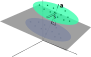
\includegraphics[width=0.75\columnwidth]{illustration_classification}
			\caption{{\bf Input Space for a Simple Linear Classification Task.}
				Two clusters of presynaptic basal activity were generated from 
				multivariate Gaussian distributions. Here, $s$ denotes the standard
				deviation orthogonal to the normal vector of the classification
				hyperplane.}
			\label{fig:illustration_classification}
		\end{figure}
		%%%%%%%%%%%%%%%%%%%%%%%%%%%%%%%%%%%%%
		
		For the classification task, we set up two output neurons receiving
		the same basal presynaptic input, while the top-down input encoded
		the correct linear classification in a one-hot scheme, that is
		%%%%%%%%%%%%%%%%%%%%%%%%%%%%%%%%%%%%%
		\begin{align}
			x_{d,0}(t) &= 1 - \Theta\left( \left(\mathbf{x}_p(t) - \mathbf{b}\right)^T \mathbf{a}\right) \\
			x_{d,1}(t) &= \Theta\left( \left(\mathbf{x}_p(t) - \mathbf{b}\right)^T \mathbf{a}\right) \; ,
		\end{align}
		%%%%%%%%%%%%%%%%%%%%%%%%%%%%%%%%%%%%%
		where $\Theta(x)$ is the Heaviside step function.
		
		As in the previous experiment, we ran a full simulation until 
		all dynamic variables reached a stationary state. After this,
		a test run without plasticity and with the apical input turned off 
		was used to evaluate the classification	performance. For each sample,
		the index of the neuron with the highest activity was used
		as the predicted class. Accuracy was then calculated as the fraction
		of correctly classified samples.
		%%%%%%%%%%%%%%%%%%%%%%%%%%%%%%%%%%%%%
		\begin{figure}
			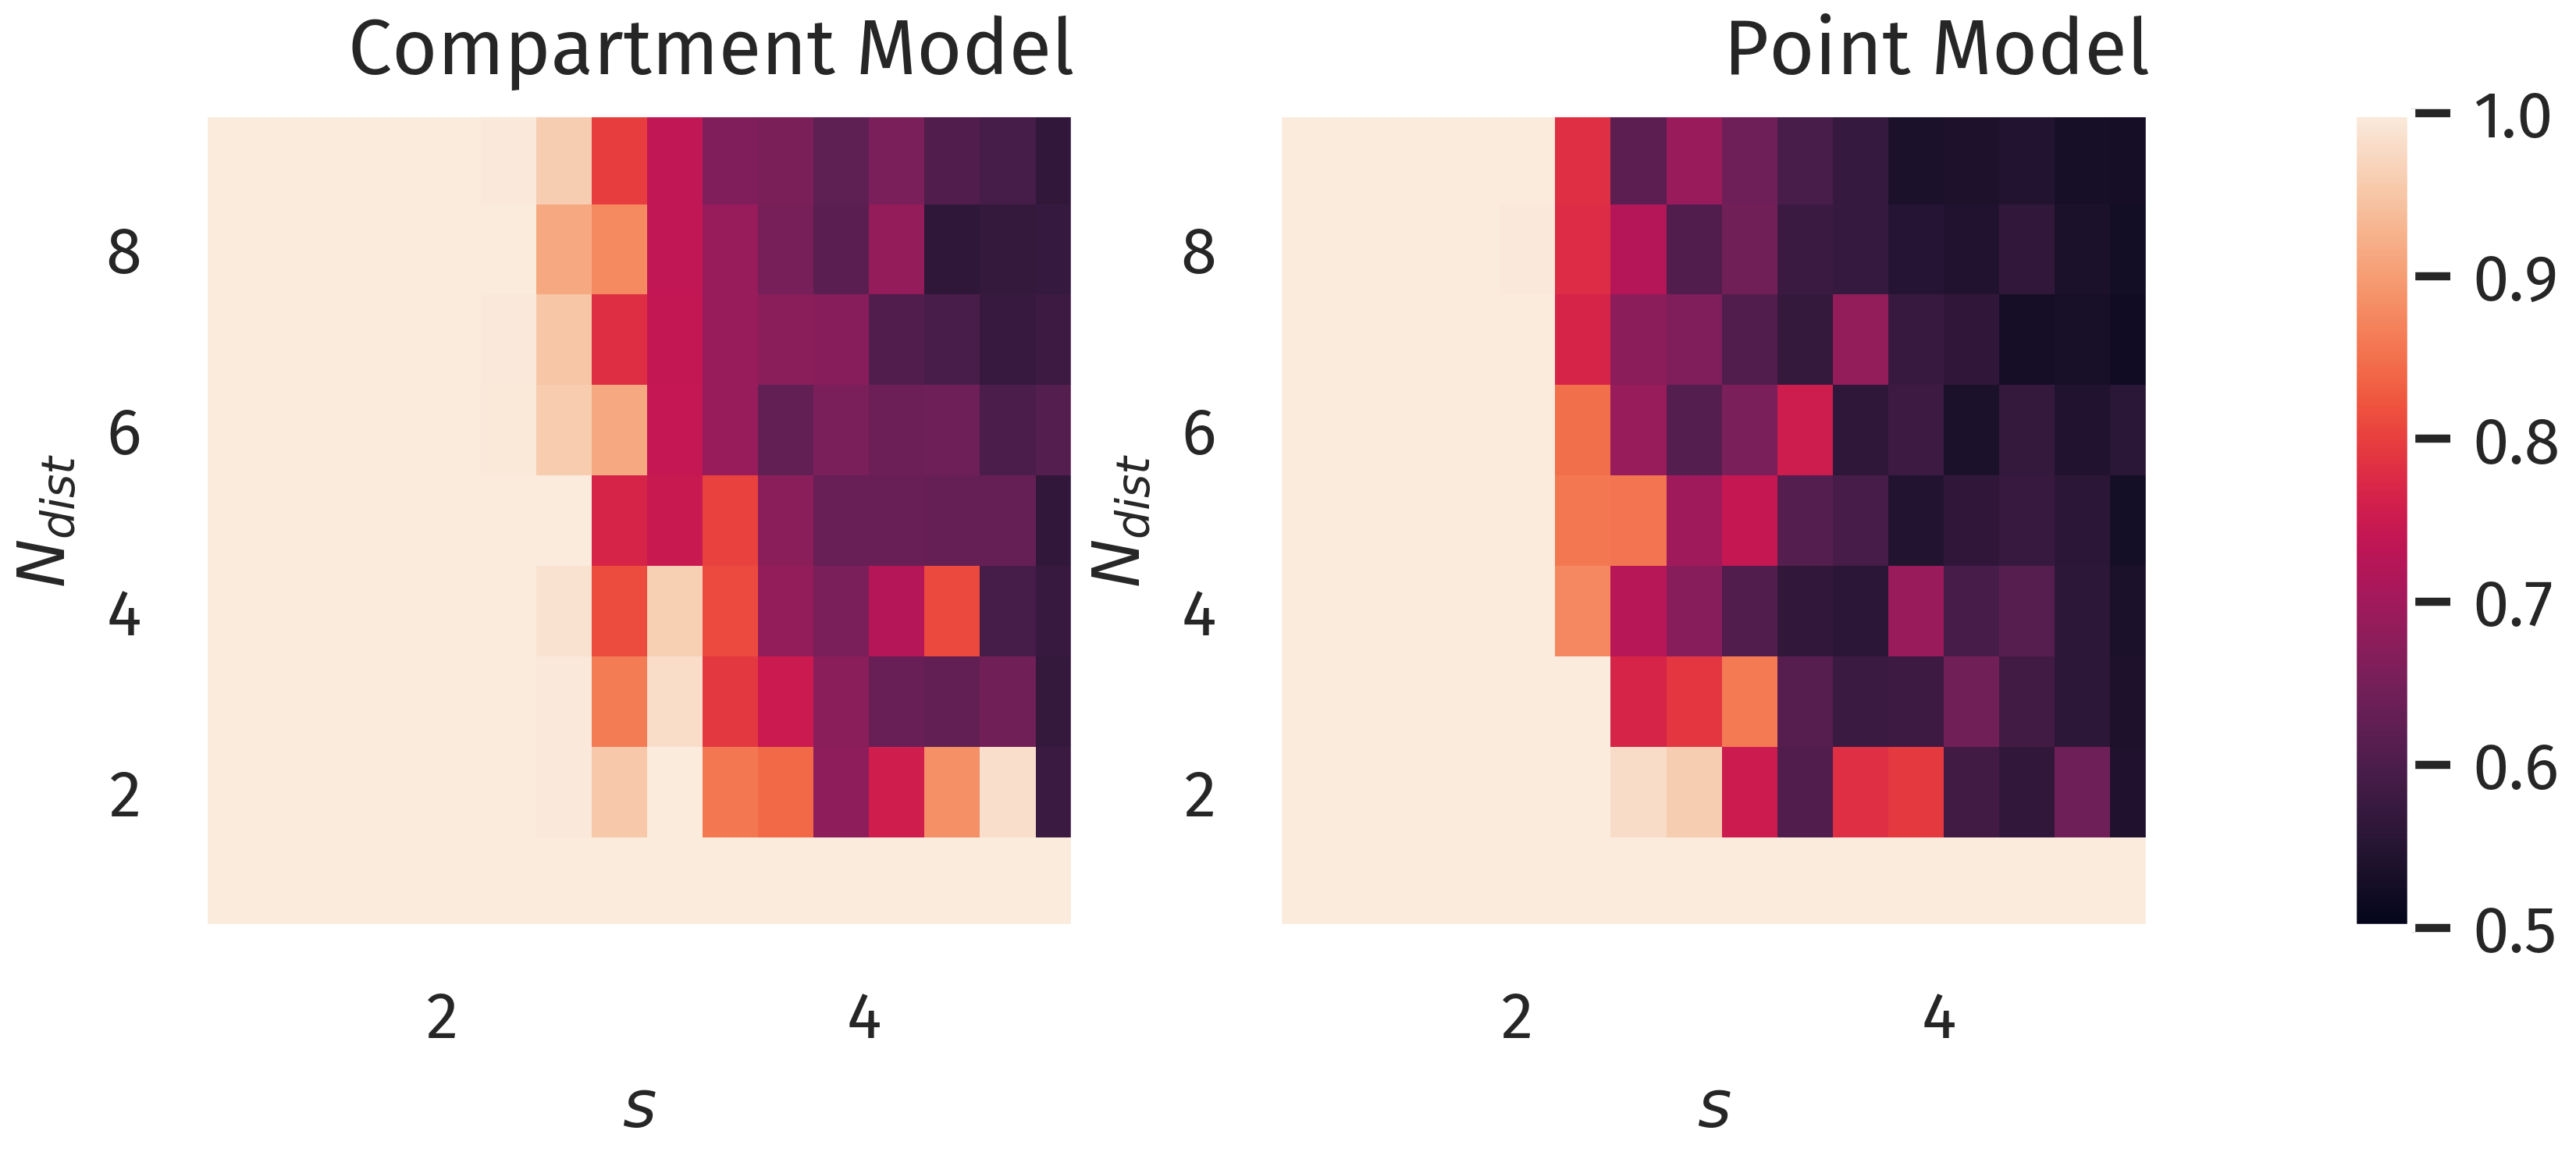
\includegraphics[width=\columnwidth]{classification_dimension_scaling}
			\caption{{\bf Binary Classification Accuracy.}
			Fraction of correctly classified patterns as illustrated in
			Fig.~\ref{fig:illustration_classification}, see 
			Section~\ref{sect:classification}.¸}
		\label{fig:classification_accuracy}
		\end{figure}
		%%%%%%%%%%%%%%%%%%%%%%%%%%%%%%%%%%%%%
		
		The resulting accuracy as a function of $N_{dist}$ and $s$
		is shown in Fig.~\ref{fig:classification_accuracy}.
		Albeit differences are small, the compartment model does
		show a better overall accuracy for the tested parameter range.
		
		\subsection{Non-Hebbian Learning Rules}
		\label{sect:non-hebbian}
		
		Instead of Hebbian learning, we also considered a BCM-like
		learning rule for the basal weights \citep{Bienenstock1982,Intrator1992}.
		The form of the BCM-rule we consider here reads
		%%%%%%%%%%%%%%%%%%%%%%%%%%%%%%%%%%%%%
		\begin{equation}
		\Delta w_i \propto y\left(y - \theta_M\right) x_i - \epsilon w_i \; ,
		\end{equation}
		%%%%%%%%%%%%%%%%%%%%%%%%%%%%%%%%%%%%%
		where $\theta_M$ is a threshold defining a transition from LTP to LTD and
		$\epsilon$ is an optional decay term on the weights.
		In the variant introduced by \citet{Law1994}, the sliding threshold is simply
		the temporal average of the squared neural activity, 
		$\theta_M = \langle y^2 \rangle$. In practice, this would be calculated
		as a running average, thereby preventing the weights from growing 
		indefinitely.
		
		However, for our compartment model, we chose to explicitly set the
		threshold to be the mean value between the high- and low-activity regime
		in our compartment model, i.e.\ $\theta_M = (1+\alpha)/2$. By doing so, LTP is
		preferably induced if both basal and apical input are present at the same
		time. Furthermore, instead of the weight decay term, we chose to keep
		the weight normalization as introduced in \eqref{eq:weight_norm}.
		Obviously, for the point model, the reasoning behind our choice of
		$\theta_M$ did not apply. Still, to provide some level of comparability,
		we also ran simulations with a point model where the sliding threshold was
		calculated as a running average of $y^2$. Furthermore, we did not use
		weight normalization in this case, but chose to use a small weight decay term
		with $\epsilon = 0.1$. The results are shown in 
		Fig.~\ref{fig:classification_accuracy_bcm} (classification task) and 
		Fig.~\ref{fig:classification_accuracy_bcm} (Basal-Apical alignment). 
		While the accuracy of the classification for the point model
		is at most comparable to Hebbian learning, the BCM-like rule for the 
		compartment model significantly increases the accuracy for the tested
		parameter range (compare Fig.~\ref{fig:classification_accuracy}).
		
		Likewise, the compartment model significantly benefits from
		the BCM rule in terms of basal-apical alignment, while only marginal
		improvements can be observed for the point model
		(compare Fig.~\ref{fig:corr_dimension_scaling_bcm} 
		with Fig.~\ref{fig:corr_dimension_scaling}).
		
		%%%%%%%%%%%%%%%%%%%%%%%%%%%%%%%%%%%%%
		\begin{figure}
			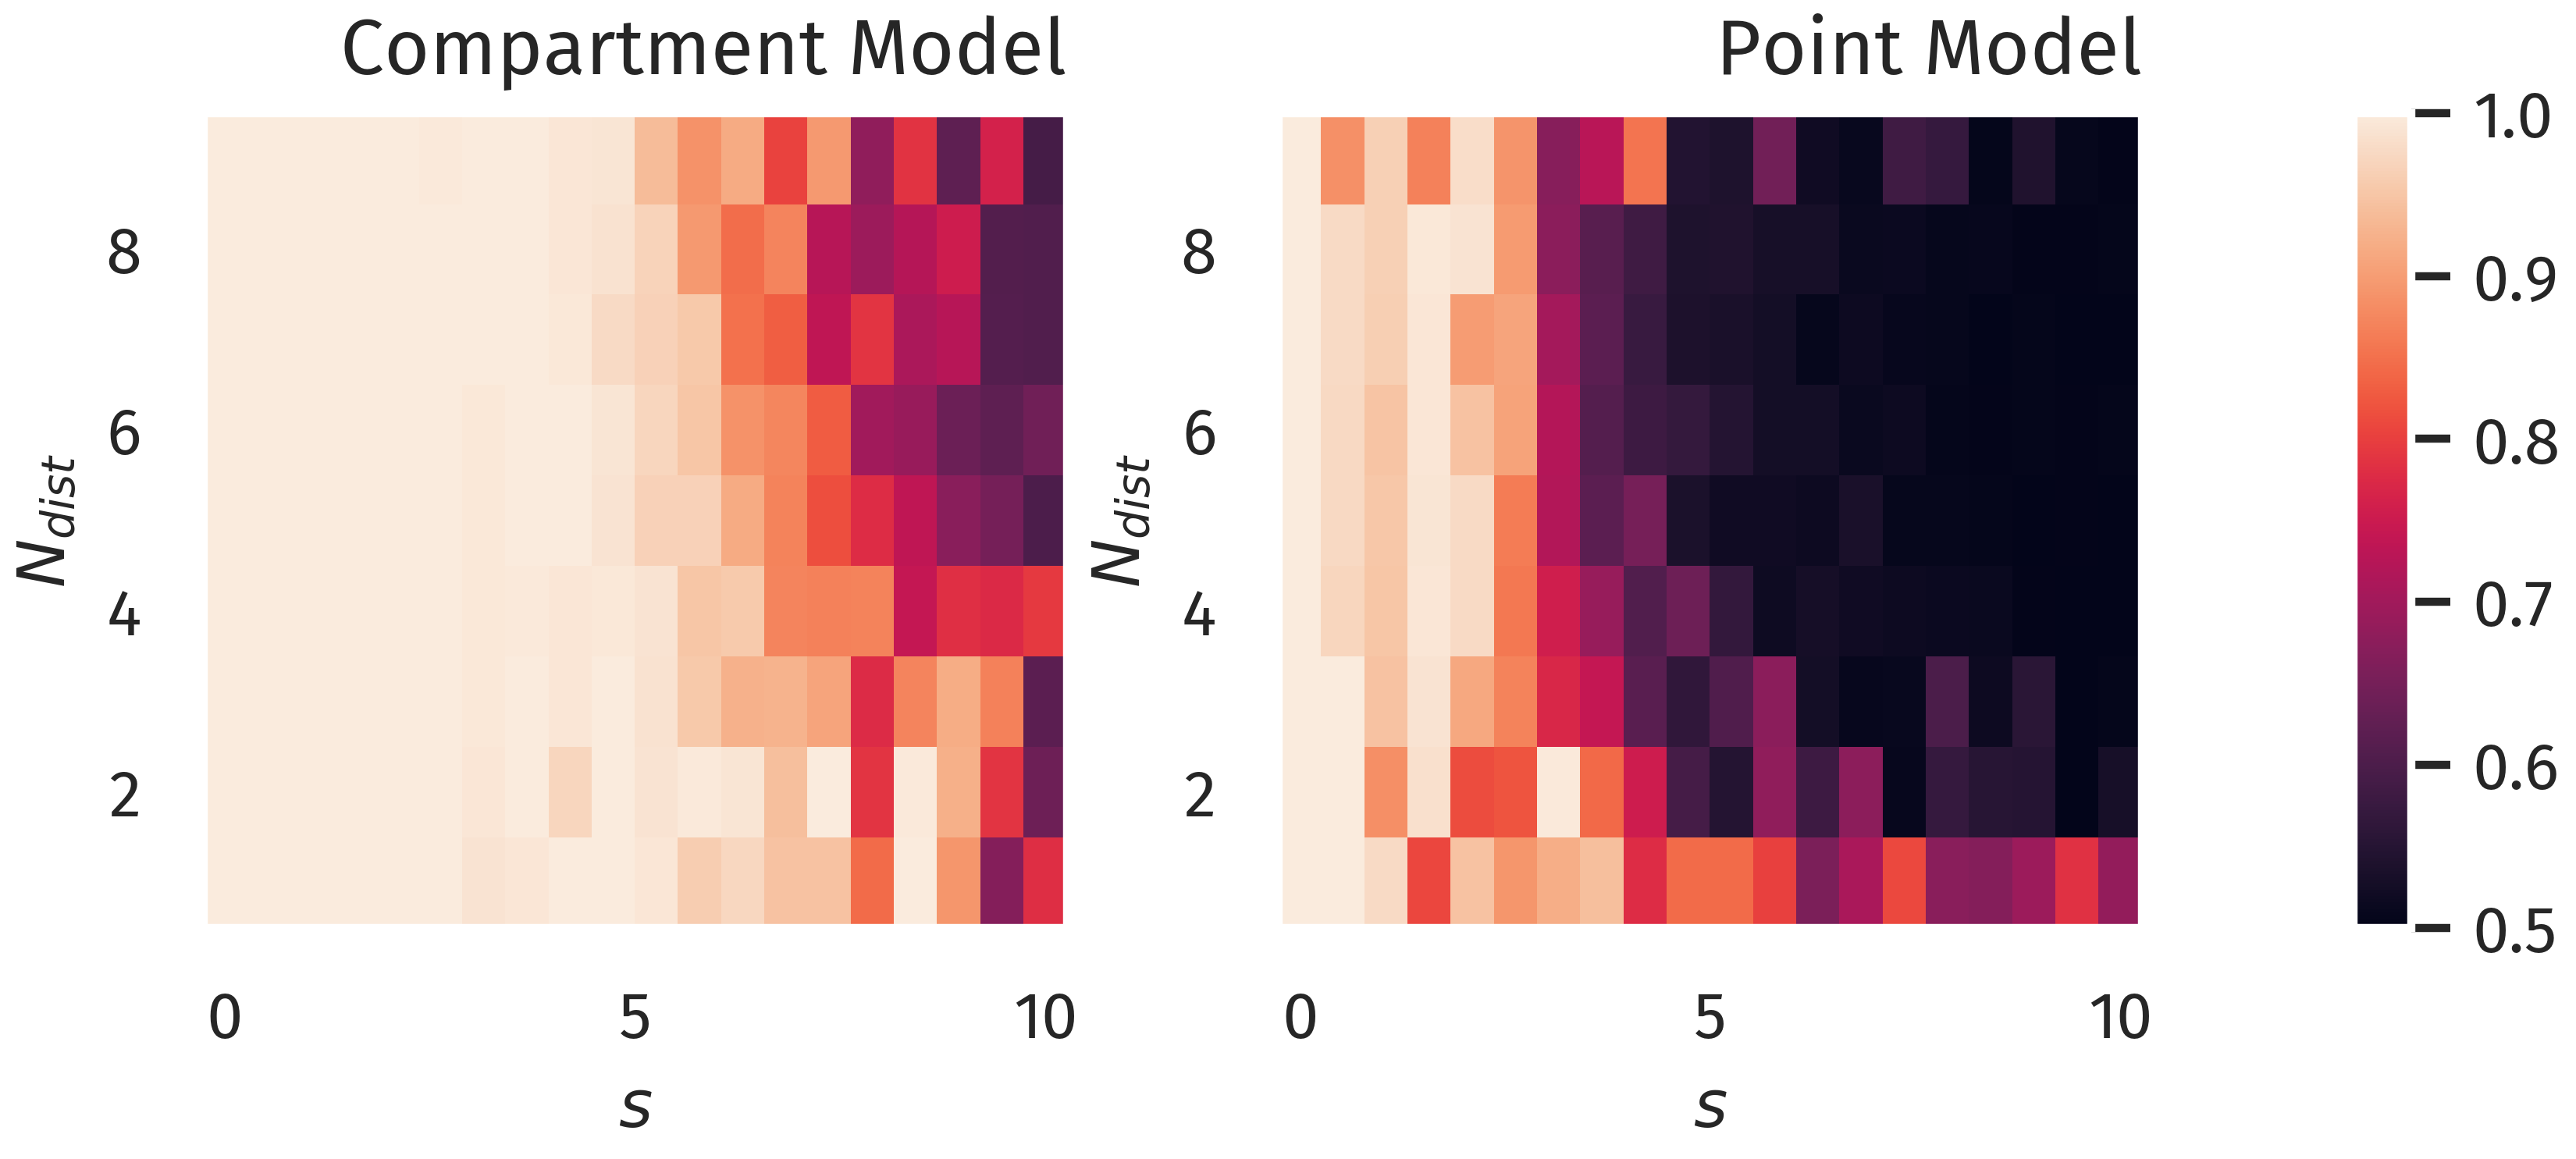
\includegraphics[width=\columnwidth]{classification_dimension_scaling_bcm}
			\caption{{\bf Binary Classification Accuracy, BCM Rule.}
				Fraction of correctly classified patterns as illustrated in
				Fig.~\ref{fig:illustration_classification}, after training with
				a BCM-like learning rule.¸}
			\label{fig:classification_accuracy_bcm}
		\end{figure}
		%%%%%%%%%%%%%%%%%%%%%%%%%%%%%%%%%%%%%
		
		%%%%%%%%%%%%%%%%%%%%%%%%%%%%%%%%%%%%%
		\begin{figure}
			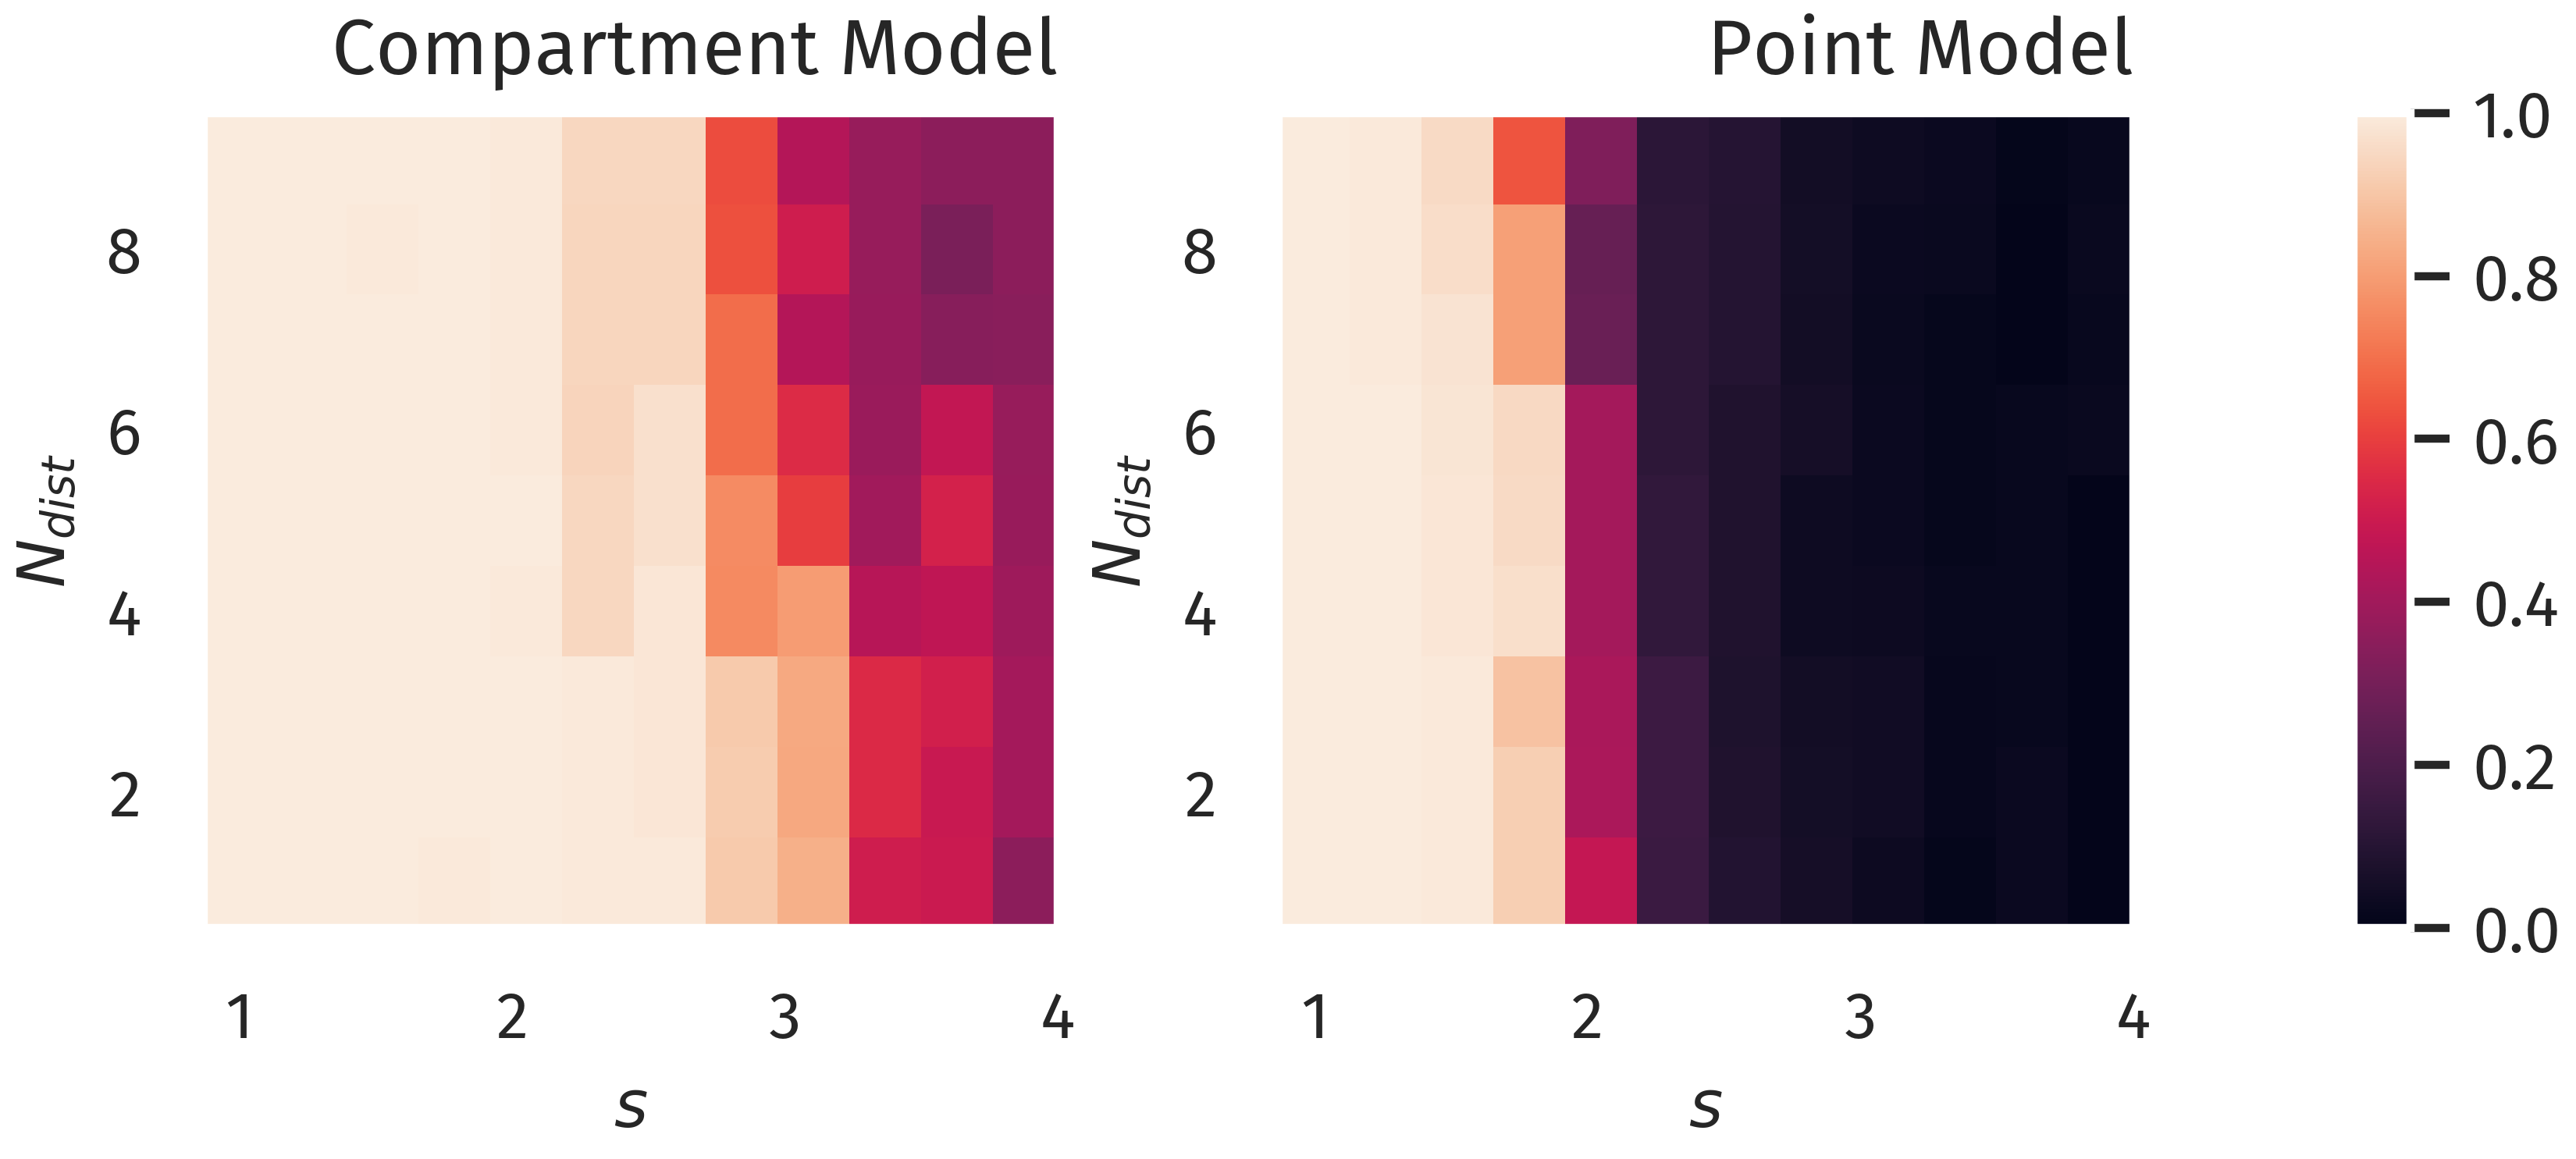
\includegraphics[width=\columnwidth]{corr_dimension_scaling_bcm}
			\caption{{\bf Alignment between Basal and Apical Input, BCM Rule.}
				Color encodes the Pearson correlation $\rho[I_p,I_d]$ for different
				number of orthogonal distraction directions $N_{dist}$ 
				and the corresponding scaling faction $s$ after training
				with a BCM-like rule. Compare to Fig.~\ref{fig:corr_dimension_scaling}.}
			\label{fig:corr_dimension_scaling_bcm}
		\end{figure}
		%%%%%%%%%%%%%%%%%%%%%%%%%%%%%%%%%%%%%
		
		\section{Discussion}
		
		To be continued
		
		
		\bibliography{Dendritic_Learning}
		
\end{document}